\section{Evaluation}

\begin{frame}
    \frametitle{Counting crates with UB (1/2)}
    {\footnotesize
    Data obtained using \href{https://github.com/saethlin/miri-tools}{\texttt{github:saethlin/miri-tools}}\\
    }
    \begin{figure}
        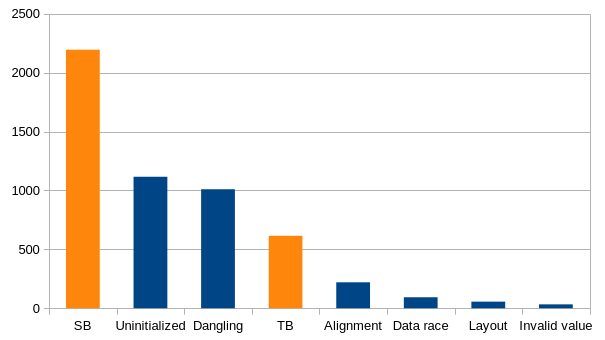
\includegraphics[width=0.8\textwidth]{../img/ub-count.png}
    \end{figure}
    {\footnotesize Number of crates on \texttt{crates.io} with at least one test
    that contains UB, for each kind of UB detected by Miri.}\\~\\
\end{frame}

\begin{frame}
    \frametitle{Counting crates with UB (2/2)}
    \begin{tabular}{|l|c|c|l|}
        \hline
        Kind                         &  SB &  TB & Notes\\
        \hline
        Protector invalidations      &  70 &  58 & \tiny(1) \\
        Protector deallocations      &  12 &  12 & \\
        Accesses without permissions & 998 & 545 & \tiny(2) \\
        Accesses outside range       & 903 &   0 & \tiny(3) \\
        Wildcard pointers            & 213 & --- & \tiny(4) \\
        \hline
    \end{tabular}~\\~\\
    From 97~851 crates, of which 3~808 contain UB of any kind\\~\\

    {\footnotesize
    \(^{(1)}\) now allowed: \texttt{Reserved -> Frozen}\\
    \(^{(2)}\) see: \texttt{as\_mut\_ptr}\\
    \(^{(3)}\) not included: accesses in wrong allocation\\
    \(^{(4)}\) not handled by TB\\
    }
\end{frame}

\begin{frame}
    \frametitle{Notable examples}
    \begin{block}{Accesses outside range}
        UB in \texttt{tokio}, \texttt{pyo3}, \texttt{rkyv}, \texttt{eyre}, \texttt{ndarray}, ...\\
        according to SB but not TB
    \end{block}
    \begin{block}{Invalidations by mutable reborrows (``\texttt{as\_mut\_ptr}'' pattern)}
        UB in \texttt{arrayvec}, \texttt{slotmap}, \texttt{nalgebra}, \texttt{json}, ...\\
        according to SB but not TB
    \end{block}
    \begin{block}{Grepping \texttt{as\_mut\_ptr} in error logs}
        \begin{description}
            \item[SB:] 12226
            \item[TB:] 3252
        \end{description}
        {\scriptsize\texttt{rg as\_mut\_ptr logs/ ---count-matches ---no-filename | paste -s -d+ - | bc}}
    \end{block}
\end{frame}
